\section{Results and Empirical Analysis}
\label{sec:results}

\subsection{Comparative Classifier Performance}
Table~\ref{tab:model_comparison} summarizes the empirical performance of all five machine learning models on the held-out test partition ($N_{\text{test}} = 11,729$), alongside 5-fold cross-validation scores on the training set, PR-AUC, and batched inference latency.

\begin{table*}[t]
\caption{Classification Performance and Computational Latency Across Evaluated ML Models (Test Set: $N=11,729$)}
\label{tab:model_comparison}
\centering
\resizebox{\textwidth}{!}{
\begin{tabular}{lccccccccc}
\hline
\textbf{Model Architecture} & \textbf{Acc (\%)} & \textbf{Prec (\%)} & \textbf{Rec (\%)} & \textbf{F1 (\%)} & \textbf{ROC-AUC} & \textbf{PR-AUC (AP)} & \textbf{5-Fold CV F1 (\%)} & \textbf{Batch Lat (ms per 1,000 URLs)} & \textbf{Single Lat (ms)} \\
\hline
Logistic Regression & 89.97 & 89.23 & 91.91 & 90.55 & 0.9613 & 0.9637 & 90.48 $\pm$ 0.20 & 1.41 $\pm$ 0.16 & 0.30 \\
Decision Tree & 93.61 & 93.36 & 94.49 & 93.92 & 0.9668 & 0.9546 & 93.62 $\pm$ 0.17 & 0.53 $\pm$ 0.05 & 0.22 \\
Random Forest & 94.30 & 94.03 & 95.12 & 94.57 & 0.9867 & 0.9880 & 94.79 $\pm$ 0.11 & 10.60 $\pm$ 0.31 & 49.38 \\
Linear SVM & 89.99 & 89.10 & 92.12 & 90.58 & 0.9613 & 0.9637 & 90.45 $\pm$ 0.22 & 2.85 $\pm$ 0.20 & 4.01 \\
\textbf{XGBoost} & \textbf{94.82} & \textbf{94.88} & \textbf{95.22} & \textbf{95.05} & \textbf{0.9879} & \textbf{0.9889} & \textbf{95.17 $\pm$ 0.13} & \textbf{2.46 $\pm$ 0.20} & \textbf{0.71} \\
\hline
\multicolumn{10}{l}{\footnotesize * PR-AUC corresponds to Average Precision (AP). Multi-seed XGBoost evaluation (5 random seeds) yields $94.74\% \pm 0.08\%$ Acc and $94.98\% \pm 0.08\%$ F1.} \\
\end{tabular}
}
\end{table*}


Tree-based ensemble architectures demonstrate superior discriminative capability over linear baselines:
\begin{itemize}
    \item \textbf{XGBoost} achieves the highest overall performance: 94.82\% Accuracy, 94.88\% Precision, 95.22\% Recall, 95.05\% F1, 0.9879 ROC-AUC, and 0.9889 PR-AUC (5-fold CV F1: $95.17\% \pm 0.13\%$) with $2.46 \pm 0.20$\,ms batch latency per $10^3$ URLs and 0.71\,ms single-query latency ($\sim 60\times$ the 11.6\,$\mu$s feature extraction time).
    \item \textbf{Random Forest} attains 94.30\% Accuracy, 94.57\% F1, 0.9867 ROC-AUC, and 0.9880 PR-AUC (CV F1: $94.79\% \pm 0.11\%$) with $10.60 \pm 0.31$\,ms latency per $10^3$ URLs.
    \item \textbf{Decision Tree} achieves 93.61\% Accuracy, 93.92\% F1, and 0.9668 ROC-AUC (CV F1: $93.62\% \pm 0.17\%$) at $0.53 \pm 0.05$\,ms latency.
    \item \textbf{Linear Models} (Logistic Regression and Linear SVM) attain 89.97\% and 89.99\% accuracy (CV F1: $90.48\%$ and $90.45\%$). Both models produce near-identical ROC-AUC (0.9613) and PR-AUC (0.9637) when rounded to four decimals (unrounded: 0.961327 vs. 0.961293 ROC-AUC; 0.963710 vs. 0.963676 PR-AUC). This parity is directly substantiated by the high cosine similarity of their standardized coefficient vectors ($\cos(\mathbf{w}_{\text{LR}}, \mathbf{w}_{\text{SVM}}) = 0.8307$) and a near-unity rank correlation between their continuous test decision scores ($\rho_s = 0.9997$ Spearman rank correlation, Pearson $r = 0.9836$); because threshold-free ROC and PR curves depend strictly on the rank-ordering of prediction scores, near-identical test rankings generate identical rounded area metrics.
\end{itemize}

On the test set, XGBoost identifies 5,836 True Positives ($TP$) out of 6,129 phishing URLs ($\text{Recall} = 95.22\%$) and 5,285 True Negatives ($TN$) out of 5,600 benign URLs ($\text{Specificity} = 94.38\%$), with $\text{FPR} = 5.62\%$ and $\text{FNR} = 4.78\%$.

To verify whether XGBoost's performance advantage over Random Forest is statistically significant, we conducted McNemar's test with continuity correction on test predictions ($b=161$ instances where XGBoost was correct and RF incorrect; $c=100$ instances where RF was correct and XGBoost incorrect). The test yields $\chi^2 = 13.79$ ($p = 2.04 \times 10^{-4} < 0.001$), confirming statistical significance. Multi-seed evaluation across 5 random seeds (seeds 42, 123, 456, 789, 2024; varying model tree subsampling with fixed test split) confirms stability: XGBoost achieves a mean accuracy of $94.74\% \pm 0.08\%$ and a mean F1-score of $94.98\% \pm 0.08\%$ versus Random Forest's $94.59\% \pm 0.06\%$.

\begin{figure}[htbp]
\centering
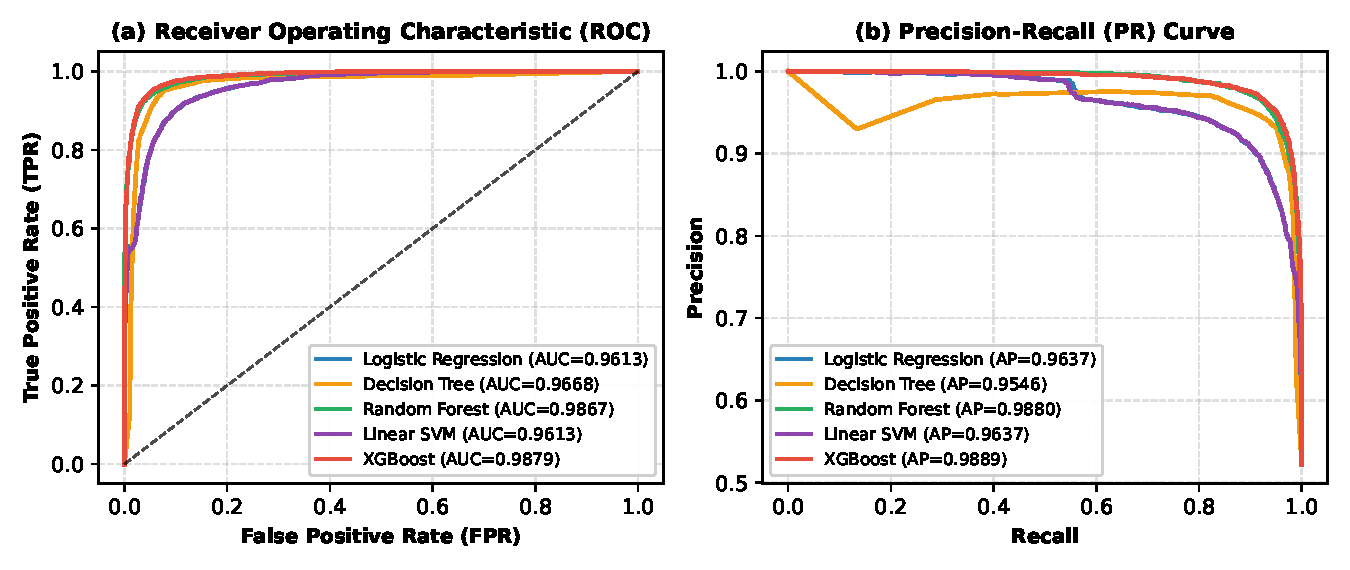
\includegraphics[width=0.88\columnwidth]{figures/fig5_roc_pr_curves.pdf}
\caption{Discrimination Diagnostics: (a) ROC Curves, and (b) Precision-Recall Curves across all evaluated classifiers.}
\label{fig:roc_pr}
\end{figure}

Fig.~\ref{fig:roc_pr} depicts the ROC and Precision-Recall (PR) curves. XGBoost and Random Forest maintain steep true positive trajectories, achieving Average Precision (AP) scores of 0.9889 and 0.9880 respectively, with Decision Tree achieving 0.9546 AP.

\subsection{Explainable AI via TreeSHAP}
TreeSHAP analysis was executed strictly on the training partition ($N=500$ random samples) to extract global feature rankings under a train-only protocol. Table~\ref{tab:shap_features} details the top 10 most influential features according to mean absolute SHAP value and plausible cybersecurity semantic rationales.

\begin{table*}[t]
\caption{Top 10 Most Influential Features Ranked by Mean Absolute TreeSHAP Value on Training Partition}
\label{tab:shap_features}
\centering
\begin{tabular}{clccp{10.5cm}}
\hline
\textbf{Rank} & \textbf{Feature Identifier} & \textbf{Modality} & \textbf{Mean $|\text{SHAP}|$} & \textbf{Plausible Cybersecurity Interpretation} \\
\hline
1 & \texttt{directory\_length} & Lexical & 1.0811 & Directory path length / presence (deep nesting often masks fraud; $-1$ indicates no path) \\
2 & \texttt{time\_domain\_activation} & Network & 0.9912 & Domain age in days (new domains and failed lookups often correlate with throwaway setups) \\
3 & \texttt{qty\_slash\_url} & Lexical & 0.7377 & Forward slash delimiter count across URL hierarchy \\
4 & \texttt{length\_url} & Lexical & 0.7222 & Raw URL character length (often used to obscure destination) \\
5 & \texttt{qty\_dot\_domain} & Lexical & 0.5293 & Subdomain dot count (frequently used in multi-level brand spoofing) \\
6 & \texttt{ttl\_hostname} & Network & 0.3147 & DNS TTL metric (short TTLs are consistent with fast-flux evasive DNS) \\
7 & \texttt{asn\_ip} & Network & 0.2057 & Autonomous System Number (differentiates bulletproof/rogue hosting ASNs) \\
8 & \texttt{time\_response} & Network & 0.1724 & HTTP response latency in seconds (reflects temporary host variability) \\
9 & \texttt{qty\_hyphen\_directory} & Lexical & 0.1277 & Hyphens in directory path (often inserted to mimic brand keywords) \\
10 & \texttt{qty\_redirects} & Network & 0.1082 & HTTP redirection hop count (multi-hop chains obscure destination landing) \\
\hline
\end{tabular}
\end{table*}


\begin{figure}[htbp]
\centering
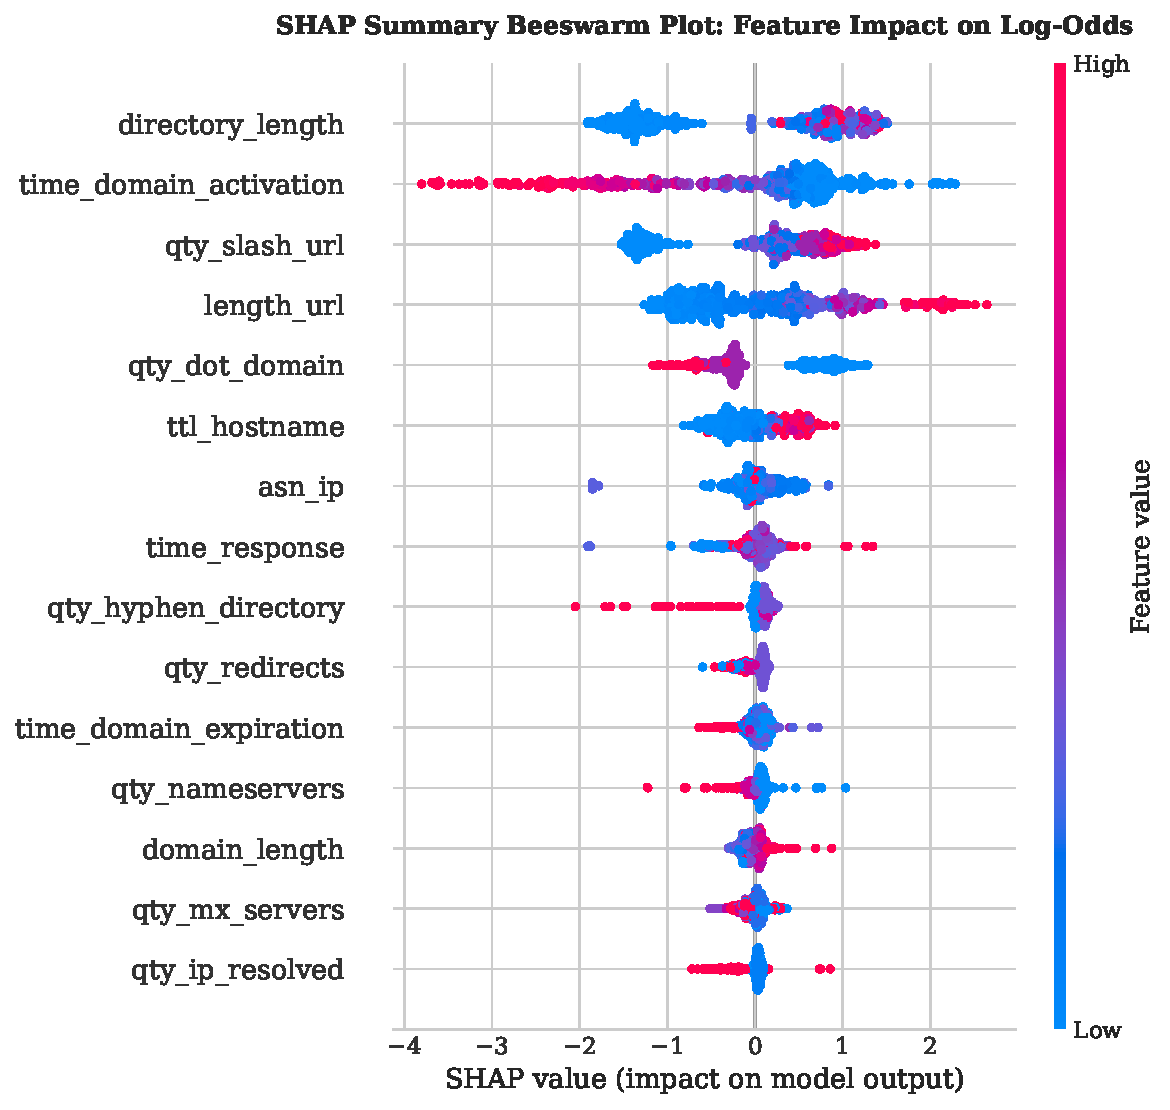
\includegraphics[width=0.88\columnwidth]{figures/fig7_shap_summary_beeswarm.pdf}
\caption{SHAP Summary Beeswarm Plot Illustrating Feature Impact Directionality on the Training Partition.}
\label{fig:shap_beeswarm}
\end{figure}

Fig.~\ref{fig:shap_beeswarm} illustrates global importance and directional attribution across training samples:
\begin{enumerate}
    \item \textbf{Directory Length (\texttt{directory\_length})}: Emerges as the top feature ($\text{Mean } |\text{SHAP}| = 1.0811$). Elongated paths (red points) shift predictions toward higher phishing log-odds. Crucially, as detailed in Section~\ref{sec:methodology}, this attribution reflects both directory depth and qualitative presence, as 60.29\% of legitimate test URLs (59.86\% in the training partition) lack paths (encoded as $-1$). Decision trees split between $-1$ (path absent) and positive lengths, effectively combining existence and magnitude into a single decision threshold.
    \item \textbf{Domain Registration Age (\texttt{time\_domain\_activation})}: Represents the second most decisive feature ($0.9912$). Mature domains correlate with negative SHAP values (legitimate signal), whereas recent domains and unresolvable WHOIS records ($-1$ sentinels) shift log-odds toward phishing, capturing throwaway infrastructure.
    \item \textbf{Delimiters and Structural Tokens (\texttt{qty\_slash\_url}, \texttt{length\_url}, \texttt{qty\_dot\_domain})}: Slash counts ($0.7377$), URL length ($0.7222$), and authority dots ($0.5293$) reflect structural obfuscation tactics commonly leveraged to evade token filters.
\end{enumerate}

\subsection{Feature Selection and Computational Benchmarking}
To assess whether compact feature subsets maintain classification performance, we evaluated XGBoost across nested feature subsets ranked by training set SHAP importance: Full (98 features), Top-30, Top-20, Top-10, Top-5, alongside a dedicated \textbf{Lexical-Only baseline} (84 features, 0 network lookups). Table~\ref{tab:feature_selection_resources} and Fig.~\ref{fig:feature_selection} delineate performance, latency, and throughput trade-offs.

\begin{table*}[t]
\caption{Impact of Feature Reduction and Computational Profile (Test Set: $N=11,729$)}
\label{tab:feature_selection_resources}
\centering
\resizebox{\textwidth}{!}{
\begin{tabular}{lccccccr}
\hline
\textbf{Configuration} & \textbf{Net / Lex} & \textbf{Acc (\%)} & \textbf{F1 (\%)} & \textbf{ROC-AUC} & \textbf{Lat (ms / $10^3$ URLs)} & \textbf{Size (MB)} & \textbf{Throughput (q/s)} \\
\hline
XGBoost (Full 98) & 14N / 84L & 94.82 & 95.05 & 0.9879 & 2.46 $\pm$ 0.20 & 0.126 & 406,318 \\
XGBoost (Top-30) & 12N / 18L & 94.74 & 94.97 & 0.9882 & 1.83 $\pm$ 0.07 & 0.134 & 546,448 \\
\textbf{XGBoost (Top-20)} & \textbf{11N / 9L} & \textbf{94.82} & \textbf{95.05} & \textbf{0.9876} & \textbf{1.67 $\pm$ 0.06} & \textbf{0.130} & \textbf{600,099} \\
XGBoost (Top-10) & 5N / 5L & 94.19 & 94.48 & 0.9859 & 1.57 $\pm$ 0.11 & 0.126 & 636,942 \\
XGBoost (Top-5) & 1N / 4L & 91.32 & 91.84 & 0.9723 & 1.59 $\pm$ 0.12 & 0.121 & 628,930 \\
\textbf{XGBoost (Lexical-84)} & \textbf{0N / 84L} & \textbf{89.68} & \textbf{90.04} & \textbf{0.9627} & \textbf{3.16 $\pm$ 0.43} & \textbf{0.342} & \textbf{316,002} \\
\hline
Random Forest & 14N / 84L & 94.30 & 94.57 & 0.9867 & 10.60 $\pm$ 0.31 & 4.068 & 94,369 \\
Decision Tree & 14N / 84L & 93.61 & 93.92 & 0.9668 & 0.53 $\pm$ 0.05 & 0.029 & 1,884,868 \\
Linear SVM & 14N / 84L & 89.99 & 90.58 & 0.9613 & 2.85 $\pm$ 0.20 & 0.006 & 350,920 \\
Logistic Regression & 14N / 84L & 89.97 & 90.55 & 0.9613 & 1.41 $\pm$ 0.16 & 0.004 & 708,898 \\
\hline
\multicolumn{8}{l}{\footnotesize * Evaluated under random seed 42. Multi-seed test evaluation for Top-20 (5 seeds) yields $94.71\% \pm 0.09\%$ Acc and $94.95\% \pm 0.08\%$ F1.} \\
\end{tabular}
}
\end{table*}


\begin{figure}[htbp]
\centering
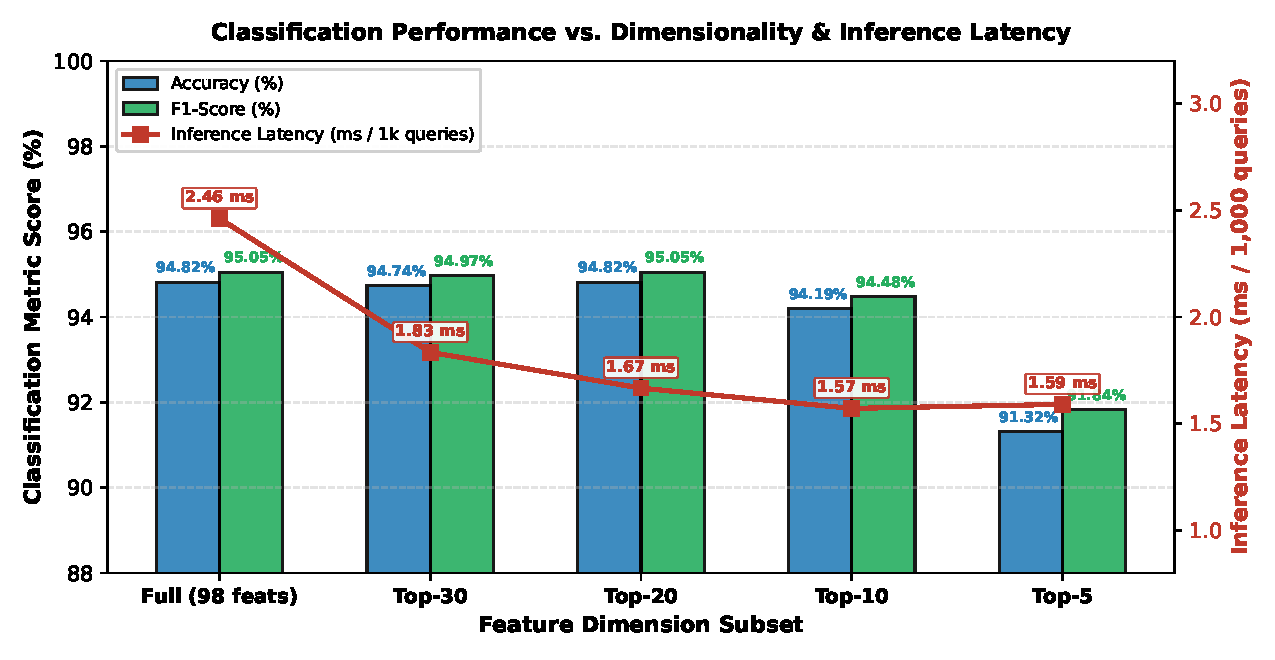
\includegraphics[width=0.88\columnwidth]{figures/fig9_feature_reduction_comparison.pdf}
\caption{Classification Performance vs. Dimensionality and Inference Latency Across Feature Subsets.}
\label{fig:feature_selection}
\end{figure}

Evaluating nested feature reduction via 5-fold cross-validation on $\mathcal{D}_{\text{train}}$ reveals progressive convergence: CV F1 increases from 91.85\% at $k=5$ and 94.52\% at $k=10$ to 95.02\% at $k=20$, 95.17\% at $k=30$, and 95.20\% at $k=98$. Although CV performance continues to edge upward at higher dimensions, we select $k=20$ as the smallest tested subset within about 0.2\,pp of full performance. Because SHAP feature rankings were computed on all of $\mathcal{D}_{\text{train}}$, top-$k$ cross-validation scores reflect mild optimism from training-set ranking reuse, whereas held-out test evaluations are strictly unbiased. Pruning the feature space to the \textbf{Top-20 subset} (a 79.6\% reduction) preserves full predictive performance: Accuracy is 94.82\%, F1-score is 95.05\%, and ROC-AUC is 0.9876 on seed 42, while multi-seed evaluation across 5 random seeds confirms stability with a test mean accuracy of $94.71\% \pm 0.09\%$, mean F1-score of $94.95\% \pm 0.08\%$, and ROC-AUC of $0.9876 \pm 0.0001$ (closely matching the full model's $94.74\% \pm 0.08\%$ and $94.98\% \pm 0.08\%$). Concurrently, model-only inference latency (excluding external network lookups) decreases from $2.46 \pm 0.20$\,ms to $1.67 \pm 0.06$\,ms per 1,000 queries in batch mode (a 32.3\% reduction; single-query latency falls to 0.46\,ms median, 0.56\,ms mean vs. 0.71\,ms for Full 98), while batch throughput increases from 406,318 to 600,099 queries/s on standard CPU hardware. The \textbf{Top-10 subset} also maintains robust efficacy with 94.19\% accuracy and 94.48\% F1-score at $1.57 \pm 0.11$\,ms latency.

Crucially, the \textbf{Lexical-Only model} achieves 89.68\% accuracy, 90.04\% F1-score, and 0.9627 ROC-AUC (CV F1: $90.19\% \pm 0.17\%$) using zero network lookups. To evaluate a practical two-tier architecture, we implemented an uncertainty-gated cascade: when the Tier 1 lexical model's predicted probability falls within an uncertainty band $[\tau_L, \tau_H]$, classification is deferred to the Tier 2 Top-20 resolver model. Operating thresholds were calibrated strictly via 5-fold cross-validation on the training set ($\mathcal{D}_{\text{train}}$) to maximize query offloading while constraining the Tier-1 out-of-fold phishing leakage rate below 2.5\% (CV sweep at $[\tau_L, \tau_H] = [0.10, 0.90]$: 64.21\% coverage, 97.98\% accuracy, 2.35\% phishing leak rate).

On the held-out test partition ($N=11,729$), Tier 1 autonomously resolves 64.28\% of instances (7,539 URLs) purely in-memory with 97.78\% accuracy, eliminating external lookups for nearly two-thirds of incoming traffic. Specifically, Tier 1 classifies 3,380 URLs as legitimate ($\hat{p} < 0.10$), of which 3,290 are true legitimate and 90 are false legitimate (phishing URLs misclassified as legitimate). This yields an empirical test leak rate of 2.66\% (90/3,380), which slightly exceeds the 2.5\% training design target due to test distribution variation. Tier 1 classifies 4,159 URLs as phishing ($\hat{p} > 0.90$), with 4,082 true phishing and 77 false alarms. Across the 4,172 phishing URLs resolved at Tier 1, 4,082 are caught, yielding a conditional Tier-1 phishing recall of 97.84\% (4,082/4,172); however, this conditional metric excludes the 1,957 phishing URLs deferred to Tier 2.

Evaluating end-to-end cascade performance across all 11,729 test instances—where the 4,190 deferred ambiguous cases are evaluated by Tier 2, which attains 88.78\% accuracy on these difficult instances—the cascade achieves an overall Accuracy of 94.57\% and F1-score of 94.81\% ($TP=5,824$, $TN=5,268$, $FP=332$, $FN=305$). The end-to-end cascade False Negative Rate is $\text{FNR} = 4.98\%$ (305 / 6,129) and False Positive Rate is $\text{FPR} = 5.93\%$ (332 / 5,600), trailing the monolithic full-feature model ($\text{FNR} = 4.78\%$, $\text{FPR} = 5.62\%$) by 0.20\,pp and 0.31\,pp while eliminating 64.28\% of external resolver queries. Thus, rather than establishing absolute superiority, the results support a tiered design whose operational benefit is offloading network queries at the cost of a modest error increase. Under a narrower deferral band $[\tau_L, \tau_H] = [0.15, 0.85]$ (providing wider autonomous decision regions), 73.1\% of queries are resolved at Tier 1 with 96.93\% accuracy (94.42\% overall accuracy).

Analyzing Tier 1 resolutions by path presence reveals both operational efficiency and a security vulnerability: Tier 1 resolves 3,051 legitimate root URLs lacking paths, 316 legitimate URLs with paths, 4,083 phishing URLs with paths, and 89 pathless phishing URLs. Critically, 88 of the 141 pathless phishing URLs in the test set (62.4\%) are misclassified as legitimate at Tier 1 ($\hat{p} < 0.10$) and never reach Tier 2, as attackers using apex root domains without path tokens evade lexical filtering. 

As a trivial comparison baseline, a heuristic classifying URLs as phishing whenever a directory path exists (\texttt{directory\_length} $> -1$) achieves 79.84\% accuracy, 83.51\% F1-score, and 97.70\% recall, capitalizing on dataset sampling skew (97.70\% of phishing vs 39.71\% of legitimate URLs contain paths). To verify whether XGBoost learns true discriminative patterns beyond this sampling artifact, we evaluate performance separately on path-bearing and pathless test subsets: on the 8,212 path-bearing URLs (where 5,988 phishing and 2,224 legitimate URLs reside, rendering naive path heuristics ineffective with only 72.92\% accuracy), full XGBoost achieves 93.59\% accuracy, 96.34\% recall, 94.95\% precision, and 95.64\% F1-score ($TN=1,917$, $FP=307$, $FN=219$, $TP=5,769$). On the 3,517 pathless URLs (141 phishing and 3,376 legitimate), monolithic XGBoost catches only 47.52\% of pathless phishing (67 of 141; $\text{Recall} = 47.52\%$, $\text{F1} = 62.04\%$), achieving 97.67\% accuracy and 99.76\% specificity ($TN=3,368$, $FP=8$, $FN=74$, $TP=67$). Notably, this 97.67\% pathless accuracy stands merely 1.68 percentage points above the all-legitimate baseline of 95.99\% (predicting all 3,517 pathless URLs as legitimate yields 95.99\% accuracy). Furthermore, an ablation removing all 56 directory, file, and parameter features—yielding a 28-feature model with no path/file/query-group features (though general length and slash counts still partially encode path presence)—attains 89.17\% accuracy (86.23\% on path-bearing, 96.05\% on pathless) and 89.58\% F1-score. When deployed in Tier 1 of the cascade at $[0.10, 0.90]$, this model resolves 62.48\% of test queries (7,328 URLs) with 97.69\% accuracy, sustaining 94.53\% overall cascade accuracy and 94.78\% F1-score, confirming that non-path lexical features reduce reliance on explicit path tokens while still supporting a tiered design.

